% This file was created with matplot2tikz v0.4.0.
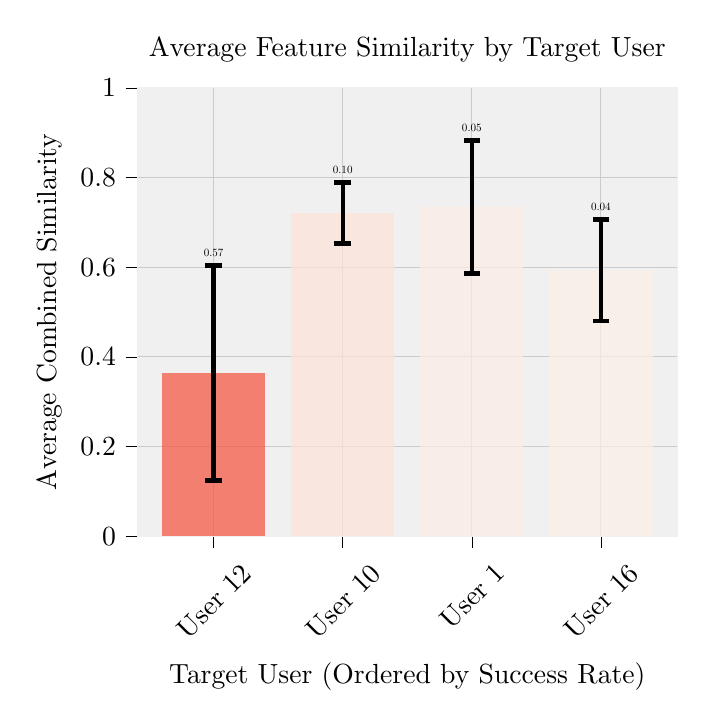
\begin{tikzpicture}

\definecolor{antiquewhite254228216}{RGB}{254,228,216}
\definecolor{lightgray203}{RGB}{203,203,203}
\definecolor{linen254237228}{RGB}{254,237,228}
\definecolor{linen254239231}{RGB}{254,239,231}
\definecolor{tomato2448057}{RGB}{244,80,57}
\definecolor{whitesmoke240}{RGB}{240,240,240}

\begin{axis}[
axis background/.style={fill=whitesmoke240},
axis line style={whitesmoke240},
tick align=outside,
tick pos=left,
title={Average Feature Similarity by Target User},
x grid style={lightgray203},
xlabel={Target User (Ordered by Success Rate)},
xmajorgrids,
xmin=-0.59, xmax=3.59,
xtick style={color=black},
xtick={0,1,2,3},
xticklabel style={rotate=45.0},
xticklabels={User 12,User 10,User 1,User 16},
y grid style={lightgray203},
ylabel={Average Combined Similarity},
ymajorgrids,
ymin=0, ymax=1,
ytick style={color=black}
]
\draw[draw=none,fill=tomato2448057,fill opacity=0.7,very thin] (axis cs:-0.4,0) rectangle (axis cs:0.4,0.364090720793222);
\draw[draw=none,fill=antiquewhite254228216,fill opacity=0.7,very thin] (axis cs:0.6,0) rectangle (axis cs:1.4,0.720677639180198);
\draw[draw=none,fill=linen254237228,fill opacity=0.7,very thin] (axis cs:1.6,0) rectangle (axis cs:2.4,0.734426309224455);
\draw[draw=none,fill=linen254239231,fill opacity=0.7,very thin] (axis cs:2.6,0) rectangle (axis cs:3.4,0.593081843040079);
\path [draw=black, ultra thick]
(axis cs:0,0.124381906961364)
--(axis cs:0,0.60379953462508);

\path [draw=black, ultra thick]
(axis cs:1,0.65239877745657)
--(axis cs:1,0.788956500903826);

\path [draw=black, ultra thick]
(axis cs:2,0.586063470819463)
--(axis cs:2,0.882789147629448);

\path [draw=black, ultra thick]
(axis cs:3,0.4801431968986)
--(axis cs:3,0.706020489181559);

\addplot [ultra thick, black, mark=-, mark size=3, mark options={solid}, only marks]
table {%
0 0.124381906961364
1 0.65239877745657
2 0.586063470819463
3 0.4801431968986
};
\addplot [ultra thick, black, mark=-, mark size=3, mark options={solid}, only marks]
table {%
0 0.60379953462508
1 0.788956500903826
2 0.882789147629448
3 0.706020489181559
};
\draw (axis cs:0,0.62379953462508) node[
  scale=0.4,
  anchor=base,
  text=black,
  rotate=0.0
]{0.57};
\draw (axis cs:1,0.808956500903826) node[
  scale=0.4,
  anchor=base,
  text=black,
  rotate=0.0
]{0.10};
\draw (axis cs:2,0.902789147629448) node[
  scale=0.4,
  anchor=base,
  text=black,
  rotate=0.0
]{0.05};
\draw (axis cs:3,0.726020489181559) node[
  scale=0.4,
  anchor=base,
  text=black,
  rotate=0.0
]{0.04};
\end{axis}

\end{tikzpicture}
